\documentclass[12pt, a4paper]{article}

% Packages
\usepackage[utf8]{inputenc}
\usepackage{geometry}
\geometry{a4paper, margin=1in}
\usepackage{amsmath, amssymb}
\usepackage{graphicx}
\usepackage{hyperref}
\usepackage{listings}
\usepackage{xcolor}
\usepackage{tikz}
\usepackage{booktabs}
\usepackage{caption}

% Color definitions for code
\definecolor{codegreen}{rgb}{0,0.6,0}
\definecolor{codegray}{rgb}{0.5,0.5,0.5}
\definecolor{codepurple}{rgb}{0.58,0,0.82}
\definecolor{backcolour}{rgb}{0.95,0.95,0.92}

\lstdefinestyle{mystyle}{
    backgroundcolor=\color{backcolour},   
    commentstyle=\color{codegreen},
    keywordstyle=\color{magenta},
    numberstyle=\tiny\color{codegray},
    stringstyle=\color{codepurple},
    basicstyle=\ttfamily\footnotesize,
    breakatwhitespace=false,         
    breaklines=true,                 
    captionpos=b,                    
    keepspaces=true,                 
    numbers=left,                    
    numbersep=5pt,                  
    showspaces=false,                
    showstringspaces=false,
    showtabs=false,                  
    tabsize=2
}
\lstset{style=mystyle}

% Title Information
\title{\textbf{Compiler Construction Report}\\
\large Architecture and Implementation of the Quantum Framework Transpiler\\
(Qiskit, Cirq, PennyLane to OpenQASM 3.0)}
\author{QCanvas Development Team}
\date{\today}

\begin{document}

\maketitle

\begin{abstract}
This report details the compiler construction principles applied to the transpilation pipeline of the QCanvas platform. The platform implements a source-to-source compiler (transpiler) that translates quantum circuits written in Python dialects of three major quantum frameworks (Qiskit, Cirq, and PennyLane) into standardized OpenQASM 3.0. By framing the transpiler within the classical phases of compiler design---Lexical Analysis, Syntax Parsing, Semantic Analysis, Intermediate Representation (IR), and Target Code Generation---this report provides a comprehensive overview of how Python's built-in Abstract Syntax Tree (AST) module was leveraged to build a secure, execution-free, multi-framework quantum compiler.
\end{abstract}

\tableofcontents
\newpage

% -------------------------------------------------------------------
\section{Introduction}
\label{sec:introduction}

In traditional software engineering, compilers translate high-level programming languages into machine code. In the quantum computing ecosystem, compilers frequently perform \textbf{source-to-source translation (transpilation)} to convert high-level framework-specific code into standard assembly formats. 

The QCanvas transpiler translates quantum circuits written in proprietary frameworks---namely \textbf{Qiskit (IBM)}, \textbf{Cirq (Google)}, and \textbf{PennyLane (Xanadu)}---into \textbf{OpenQASM 3.0}, an open hardware-agnostic intermediate representation. Unlike standard transpilers that execute user code to generate circuits dynamically, our transpiler acts purely on the static source code to maintain security in cloud-hosted environments.

This report explains how our pipeline mimics a traditional compiler's phases: from reading the source code to generating the final target assembly.

% -------------------------------------------------------------------
\section{Compiler Architecture Overview}
\label{sec:architecture}

The transpiler follows a multi-pass architecture typical of modern compilers (like LLVM or GCC). The compilation pipeline is structurally separated into a \textbf{Frontend} (parsing and semantic analysis), a \textbf{Middle-end} (Intermediate Representation), and a \textbf{Backend} (code generation).

\begin{figure}[h]
\centering
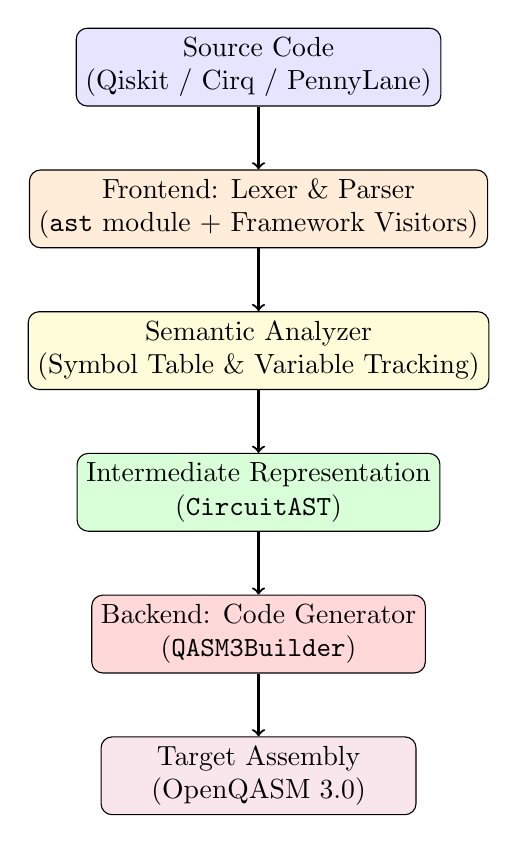
\begin{tikzpicture}[
    node distance=1.8cm,
    box/.style={rectangle, draw, rounded corners, minimum width=4cm, minimum height=0.8cm, align=center},
    arrow/.style={->, thick}
]
\node[box, fill=blue!10] (source) {Source Code\\(Qiskit / Cirq / PennyLane)};
\node[box, fill=orange!15, below of=source] (frontend) {Frontend: Lexer \& Parser\\(\texttt{ast} module + Framework Visitors)};
\node[box, fill=yellow!15, below of=frontend] (semantics) {Semantic Analyzer\\(Symbol Table \& Variable Tracking)};
\node[box, fill=green!15, below of=semantics] (ir) {Intermediate Representation\\(\texttt{CircuitAST})};
\node[box, fill=red!15, below of=ir] (backend) {Backend: Code Generator\\(\texttt{QASM3Builder})};
\node[box, fill=purple!10, below of=backend] (target) {Target Assembly\\(OpenQASM 3.0)};

\draw[arrow] (source) -- (frontend);
\draw[arrow] (frontend) -- (semantics);
\draw[arrow] (semantics) -- (ir);
\draw[arrow] (ir) -- (backend);
\draw[arrow] (backend) -- (target);
\end{tikzpicture}
\caption{The Multi-Phase Quantum Compiler Pipeline}
\label{fig:pipeline}
\end{figure}

% -------------------------------------------------------------------
\section{Phase 1: Lexical Analysis and Syntax Parsing (Frontend)}
\label{sec:frontend}

In standard compiler construction (such as with Lex and Yacc), a Lexer tokenizes the input stream and a Parser constructs an Abstract Syntax Tree (AST) based on a defined grammar. 

Because the input languages (Qiskit, Cirq, PennyLane) are effectively domain-specific languages (DSLs) embedded within Python, building a custom parser from scratch is redundant and error-prone. Instead, our compiler's frontend hooks directly into Python's native \texttt{ast} module.

\subsection{Lexing and Parsing}
The source code is ingested as a string and converted into a generic Python AST using \texttt{ast.parse()}. This inherently validates the lexical and syntactic correctness of the Python syntax before any quantum-specific compilation occurs.

\subsection{Framework-Specific AST Visitors}
Once the Python AST is generated, we employ the \textbf{Visitor Pattern} to traverse it. We implemented three separate parsers: \texttt{QiskitASTVisitor}, \texttt{CirqASTVisitor}, and \texttt{PennyLaneASTVisitor}. These visitors extract domain-specific semantics from the generic Python AST nodes.

For example, when traversing Qiskit code, the visitor intercepts assignments to detect \texttt{QuantumCircuit} initialization and intercepts expression nodes to process gate method calls.

\begin{lstlisting}[language=Python, caption=Extracting QuantumCircuit and Gate calls (qiskit\_parser.py)]
class QiskitASTVisitor(ast.NodeVisitor):
    def visit_Assign(self, node: ast.Assign) -> None:
        # Check if assigning a QuantumCircuit
        if isinstance(node.value, ast.Call) and self._is_quantum_circuit_call(node.value):
            self._extract_circuit_dimensions(node.value)
            if isinstance(node.targets[0], ast.Name):
                self.circuit_vars.add(node.targets[0].id)
                
    def visit_Expr(self, node: ast.Expr) -> None:
        # Handle expression statements, typically gate method calls like qc.h(0)
        if isinstance(node.value, ast.Call) and isinstance(node.value.func, ast.Attribute):
            self._handle_circuit_method_call(node.value)
        self.generic_visit(node)
\end{lstlisting}

% -------------------------------------------------------------------
\section{Phase 2: Semantic Analysis and Symbol Table}
\label{sec:semantics}

Semantic analysis ensures that the parsed syntactic structures have correct meaning and context. In our transpiler, semantic analysis is responsible for variable resolution, resolving dynamic loop bounds, and managing state across the AST traversal.

\subsection{The Symbol Table}
We maintain a state dictionary (symbol table) mapping variable identifiers to their resolved values. When the visitor encounters an assignment (e.g., \texttt{n\_qubits = 4}), it stores this mapping. 

\subsection{Variable Tracking and Type Resolution}
Quantum loops heavily utilize variables (e.g., \texttt{for i in range(n\_qubits): qc.h(i)}). Our semantic analyzer tracks:
\begin{itemize}
    \item \textbf{Loop Variables}: It resolves \texttt{i} within the scope of the loop body.
    \item \textbf{Register Dimensions}: It dynamically figures out qubit dimensions if they are assigned to variables instead of integer literals.
    \item \textbf{Classical Bit Mappings}: It analyzes \texttt{qc.measure(q, c)} calls to infer how many classical bits are required, assigning them to the correct registers.
\end{itemize}

\begin{lstlisting}[language=Python, caption=Variable and Loop Tracking in AST Visitor]
    def visit_For(self, node: ast.For) -> None:
        loop_var = node.target.id
        range_start, range_end = self._extract_range(node.iter)

        if self._has_circuit_ops(node.body) and range_start is not None and range_end is not None:
            # Preserving control flow in the IR
            loop_body = []
            saved_operations = self.operations
            self.operations = loop_body
            
            for stmt in node.body:
                self.visit(stmt)
                
            self.operations = saved_operations
            self.operations.append(
                ForLoopNode(
                    variable=loop_var,
                    range_start=range_start,
                    range_end=range_end,
                    body=loop_body,
                )
            )
\end{lstlisting}

% -------------------------------------------------------------------
\section{Phase 3: Intermediate Representation (IR)}
\label{sec:ir}

To support $N$ source frameworks and $M$ target languages, writing $N \times M$ direct translators is inefficient. Modern compilers solve this by using an Intermediate Representation (IR). We introduced a unified \texttt{CircuitAST} as our IR.

\subsection{Structure of the CircuitAST}
The \texttt{CircuitAST} is a framework-agnostic data structure. It isolates the backend code generation from the quirks of the frontend parsers.

\begin{lstlisting}[language=Python, caption=Data structure of the IR Nodes (circuit\_ast.py)]
@dataclass
class GateNode:
    name: str
    qubits: List[int] = field(default_factory=list)
    parameters: List[Union[float, str]] = field(default_factory=list)
    modifiers: Dict[str, Any] = field(default_factory=dict)
    metadata: Dict[str, Any] = field(default_factory=dict)

@dataclass
class MeasurementNode:
    qubit: Union[int, str]
    clbit: Union[int, str]
    metadata: Dict[str, Any] = field(default_factory=dict)

@dataclass
class CircuitAST:
    qubits: int = 0
    clbits: int = 0
    operations: List[Union[GateNode, MeasurementNode, ResetNode, BarrierNode, 'ForLoopNode', 'IfStatementNode']] = field(default_factory=list)
    parameters: Dict[str, Any] = field(default_factory=dict)
    variables: Dict[str, Any] = field(default_factory=dict)
\end{lstlisting}

Every framework parser maps its operations into this unified format. Whether the input is \texttt{qc.cx(0, 1)} (Qiskit), \texttt{cirq.CNOT(q0, q1)} (Cirq), or \texttt{qml.CNOT(wires=[0, 1])} (PennyLane), it becomes a single \texttt{GateNode(name='cx', qubits=[0,1])}.

% -------------------------------------------------------------------
\section{Phase 4: Optimization and Code Translation}
\label{sec:optimization}

Before generating the final string assembly, the compiler applies translation passes to optimize and map intermediate code to the exact targets required by OpenQASM 3.0.

\subsection{Gate Mapping and The Gate Library}
Different frameworks use different names for the same unitary operations. The compiler uses a \texttt{QASM3GateLibrary} to standardize gate nomenclature. For example, a \texttt{Toffoli} gate in PennyLane and a \texttt{CCX} gate in Cirq are both lowered to the \texttt{ccx} instruction in OpenQASM.

\subsection{Expression Evaluation}
Mathematical expressions used in gate parameters (e.g., \texttt{np.pi / 2}) are evaluated and formatted through a dedicated \texttt{QASM3Expression} module. This ensures that Python-specific references to numpy constants are accurately translated into QASM-native constants (\texttt{pi / 2}).

% -------------------------------------------------------------------
\section{Phase 5: Target Code Generation (Backend)}
\label{sec:backend}

The Backend takes the optimized \texttt{CircuitAST} and emits OpenQASM 3.0 syntax. This is managed by the \texttt{QASM3Builder}.

\subsection{Code Emission Strategy}
The builder iterates over the \texttt{CircuitAST} and sequentially appends target code instructions:
\begin{enumerate}
    \item \textbf{Prologue}: Emits the file header (\texttt{OPENQASM 3.0;}) and necessary include directives (\texttt{include "stdgates.inc";}).
    \item \textbf{Declarations}: Emits qubit and classical bit registers (\texttt{qubit[N] q; bit[M] c;}).
    \item \textbf{Operations}: Translates each \texttt{GateNode} into an assembly instruction line, appending OpenQASM gate modifiers (such as \texttt{ctrl @} or \texttt{inv @}) as required.
    \item \textbf{Control Flow}: For \texttt{ControlFlowNode} elements (like For-loops or If-statements), the builder emits valid OpenQASM 3.0 block structures, applying correct indentation for readability.
\end{enumerate}

\begin{lstlisting}[language=Python, caption=Gate application inside QASM3Builder (qasm3\_builder.py)]
class QASM3Builder:
    def apply_gate(self, gate_name: str, qubits: List[str], 
                   parameters: Optional[List[str]] = None,
                   modifiers: Optional[Dict[str, Any]] = None):
        # Build OpenQASM modifier prefix (e.g., "ctrl @ inv @ ")
        modifier_str = self._build_modifier_str(modifiers)
                
        # Format parameters (e.g., "(pi/2)")
        param_str = ""
        if parameters:
            param_str = f"({', '.join(str(p) for p in parameters)})"
            
        qubit_str = ', '.join(qubits)
        
        # Complete instruction line
        gate_app = f"{modifier_str}{gate_name}{param_str} {qubit_str};"
        self.lines.append(gate_app)
\end{lstlisting}

% -------------------------------------------------------------------
\section{Phase 6: Error Handling and Fallback Mechanism}
\label{sec:errors}

A robust compiler must handle ill-formed input gracefully. 

\subsection{Syntax Errors}
If the provided code contains standard Python syntax errors, the parser immediately throws a \texttt{SyntaxError} during the AST generation phase, halting compilation.

\subsection{Unsupported Instructions}
If the semantic analyzer encounters a framework-specific function call that cannot be mapped into a \texttt{GateNode} (e.g., deeply nested metaprogramming or unsupported custom operations), it triggers an execution-based fallback. This fallback executes the script in an isolated, sandboxed environment to dynamically serialize the in-memory circuit graph, ensuring the compilation process rarely fails.

% -------------------------------------------------------------------
\section{Conclusion}
\label{sec:conclusion}

The transpilation pipeline of the QCanvas platform mirrors the rigorous architecture of a standard compiler. By segregating the logic into a framework-specific frontend, a generic Intermediate Representation (CircuitAST), and a unified backend code generator, the system achieves massive scalability. The AST-based approach entirely eliminates the security risks of execution-based compilation, providing a highly reliable and extremely fast conversion framework.

\end{document}
